\section{Conceptual Model}\label{sec:conceptual-model}

\subsection*{Introduction}

The \textit{Theoretical Background} (Section~\ref{sec:theoretical-background}) defined five constructs (EA, EA
practitioners, EA practice, RAs, and GenAI) and introduced distributed cognition
as the integrating lens. This section synthesizes those elements into a
conceptual model that frames the investigation and maps each construct
relationship to a sub-research question. The following subsections detail the
model:

\localtableofcontents\clearpage

\subsection{Model Development}

Four theoretical streams inform the model. Distributed cognition \parencite{hutchins_cognition_1995,
      hollan_distributed_2000} treats architectural work as a cognitive system
that spans human and artificial agents. When EA practitioners use GenAI, the two
form a functional system \parencite{hutchins_cognition_1995}: neither holds
the full capability alone, and the division of labour changes how the work gets
done.

Practice theory \parencite{feldman_theorizing_2011} adds that EA work consists
of recurrent patterns of action. These patterns develop through actual use, not
from technology specifications alone
\parencite{orlikowski_sociomaterial_2007}.

The sociotechnical character of EA
\parencite{saint-louis_investigation_2019, lankhorst_enterprise_2017} means that
architectural work sits inside organizational contexts. Practitioners must
navigate stakeholder perspectives, governance constraints, and external
pressures across technological and socio-technological layers
\parencite{saint-louis_investigation_2019}.

The literature on Reference Architecture \parencite{angelov_framework_2012,
      cloutier_concept_2010} shows that RA development involves continuous cycles of
abstraction, synthesis, validation, and evolution. RAs function as boundary
objects: they must be understandable to multiple stakeholders while capturing
reusable architectural knowledge \parencite{cloutier_concept_2010}.

\subsection{The Conceptual Framework}\label{sec:conceptualframework}

Figure~\ref{fig:analytical-framework} presents the conceptual framework. Four
elements connect through specific relationships that form a cycle of practice
evolution. Guidance sits at the centre as a synthesizing output that both
emerges from and feeds back into this cycle. Each relationship corresponds to a
sub-research question (sRQ1--sRQ4), as defined in
Section~\ref{subsec:sub-questions}.

\begin{figure}[htbp]
      \centering
      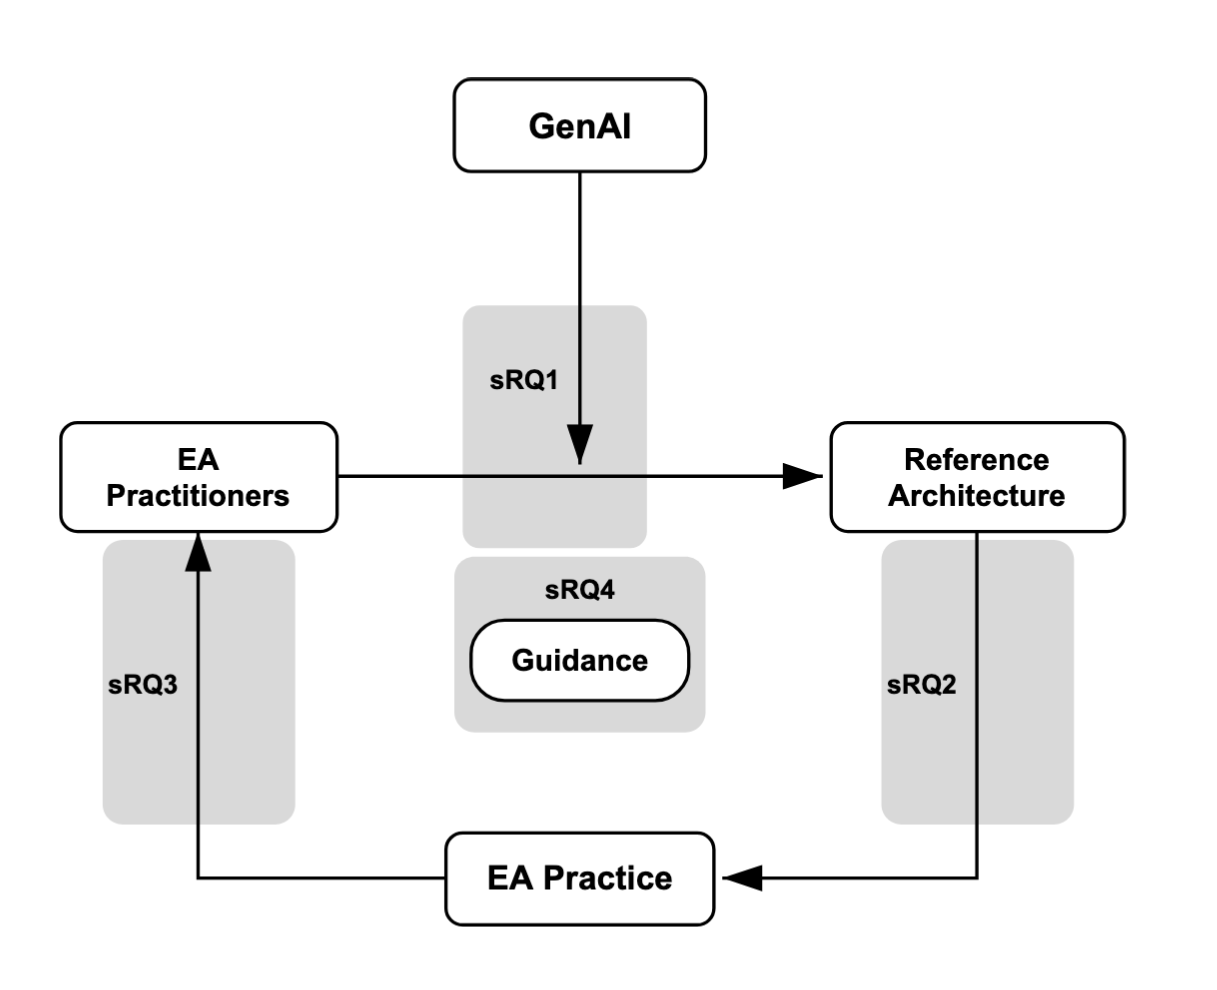
\includegraphics[width=0.7\textwidth]{images/04_1_analyticalFramework.png}
      \caption[Analytical framework for investigating EA-GenAI integration.]{Analytical Framework for Investigating EA-GenAI Integration.}
      \label{fig:analytical-framework}
\end{figure}

Elements and relationships are analysed across individual-collective, descriptive-prescriptive, and temporal dimensions (see Section~\ref{subsec:frameworkdimensions} for tractability within the Delphi design). The five core constructs (GenAI, EA Practitioners, Reference Architecture, EA
Practice, and Guidance) were defined in \textit{Core Constructs for This Study} (Section~\ref{subsec:coreelements}). The
following subsections detail the analytical dimensions and the specific
relationships between these constructs.

\subsubsection{Framework Dimensions}\label{subsec:frameworkdimensions}

Beyond the structural relationships, three analytical dimensions shape how
GenAI integration plays out in practice. Each dimension varies in how directly
the Delphi design can capture it.

\begin{enumerate}
      \item \textbf{Individual-Collective}: Distributed cognition theory
            \parencite{hutchins_cognition_1995} holds that practices develop at both
            individual and collective levels. Practitioners build personal approaches
            while contributing to shared organizational patterns. The Delphi captures
            individual practices through self-report (Round~1) and surfaces collective
            patterns through group deliberation (Rounds~2--3). It does not, however,
            collect organizational-level data; collective dynamics are inferred from
            practitioner accounts.
      \item \textbf{Descriptive-Prescriptive}: The framework separates what is
            happening now (descriptive) from what should happen (prescriptive). The
            descriptive side draws on empirical data from all three rounds. The
            prescriptive side is the researcher's synthesis of that input into a
            guidance artifact, validated through panel consensus (sRQ4) rather than
            field implementation.
      \item \textbf{Temporal}: Practices move from initial experimentation through
            pattern emergence to stabilization. Practitioners and organizations sit at
            different points on this curve. Within the study, temporal dynamics appear
            indirectly: practitioners give retrospective accounts, and the three
            rounds span roughly four months. Longitudinal observation falls outside
            the study's scope but remains an important avenue for future research.
\end{enumerate}

These dimensions are not separate layers; they cut across all elements and
relationships. The Delphi captures the individual-descriptive intersection most
directly, while collective and temporal dynamics are approximated through panel
deliberation and retrospective accounts.

\subsection{Framework Relationships and Manifestations}\label{subsec:framework-relationships}

Each sub-research question examines a specific relationship within the
framework. Understanding each relationship clarifies what the research must
capture and what the methodology must support
(Section~\ref{sec:methodology}).

The subsections below detail each relationship. For sRQ1--sRQ3, the analysis
identifies observable manifestations that inform data collection. For sRQ4, it
addresses how insights from the preceding relationships feed into actionable
guidance. Table~\ref{tab:framework-mapping} summarizes the mapping.

\begin{table}[htbp]
    \centering
    \caption{Mapping of Sub-Questions to Framework Relationships}
    \label{tab:framework-mapping}
    \begin{tabular}{|p{2cm}|p{4cm}|p{3.5cm}|p{4cm}|}
        \hline
        \textbf{Sub-Question} & \textbf{Framework Relationship} & \textbf{Research Focus} & \textbf{Methodological Requirement} \\
        \hline
        sRQ1 & GenAI $\rightarrow$ Reference Architecture (via EA Practitioners) & Current practices & Discovery of emerging patterns \\
        \hline
        sRQ2 & Reference Architecture $\rightarrow$ EA Practice & Practice changes & Capturing evolution effects \\
        \hline
        sRQ3 & EA Practice $\rightarrow$ EA Practitioners & Sense-making & Understanding interpretations \\
        \hline
        sRQ4 & All relationships $\rightarrow$ Guidance & Systematization & Consensus building \\
        \hline
    \end{tabular}
\end{table}

\subsubsection{sRQ1: EA Practitioner-AI Collaboration Patterns}

\textit{"What GenAI practices are EA practitioners currently using when developing RAs?"}
\vspace{0.5em}

This relationship examines how practitioners divide work between themselves and
GenAI when building RAs. Distributed cognition theory
\parencite{hutchins_cognition_1995} frames this as a redistribution of
cognitive labour across human and artificial agents.

Observable manifestations include: which RA activities practitioners delegate to
GenAI versus reserve for human judgment; whether GenAI is consulted continuously
or at specific lifecycle phases; how sophisticated prompt strategies have
become; and which tools or models practitioners prefer for architectural work.

These patterns develop at both individual and collective levels. Individual
experimentation feeds into shared organizational learning, though the pace
varies across practitioners and organizations.

\subsubsection{sRQ2: Artifact-Driven Practice Evolution}

\textit{"What changes to EA practice are EA practitioners experiencing when RAs are developed using GenAI?"}
\vspace{0.5em}

This relationship traces how RAs built with GenAI change broader EA practice.
Because sRQ2 asks what changes practitioners experience, the framework follows
the causal path from GenAI-augmented artifacts back into the practice context.
\textcite{angelov_framework_2012} describe a similar dynamic: reference
architectures influence the application contexts that produced them.

Manifestations include changes in both artifacts and processes. RAs developed
with GenAI may show different structural patterns, documentation styles, or
architectural approaches. Development cycles may speed up or demand new
validation steps. Governance, implementation projects, and knowledge management
practices may all shift as organizations encounter AI-augmented artifacts.

As \textcite{kotusev_enterprise_2018} observed, successful EA practices often
grow bottom-up rather than top-down. GenAI-augmented RAs can accelerate that
kind of organic evolution.

\subsubsection{sRQ3: EA Practitioner Sense-Making and Adaptation}

\textit{"How do EA practitioners make sense of impacts and trade-offs when adopting GenAI for RA development?"}
\vspace{0.5em}

This relationship captures the feedback loop: evolving EA practices shape how
practitioners interpret their situation and decide what to do next.
\textcite{orlikowski_technological_1994}'s concept of technological frames
explains how practitioners update their mental models in response to practice
changes.

Manifestations span cognitive and practical levels. Practitioners develop rules
of thumb for when GenAI adds value versus when it risks compromising
architectural quality. They build validation routines for AI-generated content.
Professional identity shifts as traditional expertise meets new orchestration
skills. Risk awareness grows as practitioners learn the limits of human-AI
collaboration.

This sense-making is collective, not only individual. Interpretations are
shared, debated, and refined within practitioner communities. The resulting
shared understanding shapes how practitioners approach future GenAI
interactions, closing the feedback loop.

\subsubsection{sRQ4: Synthesis into Guidance}

\textit{"How should effective GenAI practices for RA development be systematized into guidance for EA practitioners?"}
\vspace{0.5em}

The fourth sub-question sits at a meta-level: it draws from all three
relationships to produce prescriptive recommendations. From sRQ1, guidance
captures effective collaboration approaches. From sRQ2, it documents quality
criteria and process adaptations. From sRQ3, it incorporates practitioner wisdom
about trade-offs and challenges.

Turning descriptive findings into prescriptive guidance requires assessing
practice maturity, contextual fit, and compatibility with existing EA
frameworks. Because the transformation is researcher-led and validated through
panel consensus, the resulting prescriptions reflect collective judgment rather
than field-tested outcomes.

As \textcite{dellacqua_navigating_2023} observe, AI capability varies
unpredictably across tasks, creating a ``jagged technological frontier.'' The
guidance must accommodate this unevenness. Where practitioner consensus is
strong, directive recommendations are feasible; where it is not, guidance must
remain adaptive. The final artifact form depends on Round~3 findings.

\subsection{Framework Dynamics}\label{subsec:framework-dynamics}

The theoretical review surfaced three reasons why a simple tool-adoption lens
falls short. First, EA work is sociotechnical; it requires negotiation among
diverse stakeholders \parencite{saint-louis_investigation_2019}. Second, GenAI
redistributes cognitive work rather than automating it
\parencite{dellacqua_navigating_2023}. Third, professionals restructure their
practices around AI rather than merely using it as a faster tool
\parencite{noy_experimental_2023}.

These observations point to three dynamics that run through the framework:

\begin{enumerate}
      \item \textbf{Distributed cognition}: the capability of the practitioner-GenAI
            system exceeds what either party contributes alone
            \parencite{hutchins_cognition_1995}. GenAI provides pattern recognition
            across large knowledge spaces; practitioners provide contextual judgment
            and stakeholder awareness.
      \item \textbf{Emergent evolution}: practices arise from situated use
            \parencite{orlikowski_using_2000}, not from technology specifications.
            Initial experiments lead to new RA approaches, which shift practice
            patterns, which update practitioner understanding, which drives further
            experimentation.
      \item \textbf{Multi-level simultaneity}: individual experimentation and
            collective pattern formation happen in parallel. A single practitioner's
            GenAI session is both a personal learning event and a contribution to
            organizational knowledge.
\end{enumerate}

Because the phenomenon keeps evolving, any guidance produced must be designed
for periodic revision as collective understanding matures.
